\subsubsection{Twi'Lek}
\begin{samepage}
	\vspace{-1\baselineskip}
	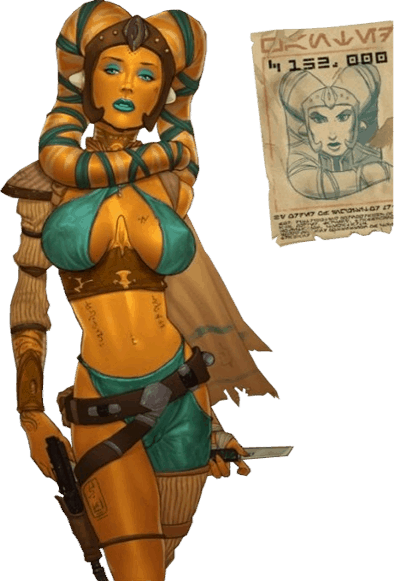
\includegraphics[width=6cm]{img/personnages/races/twilek.png}
	\vspace{-5\baselineskip}
	\begin{flushright}
		\begin{tabular}{ l l }
			\textbf{Type} 			& Humanoïde \\
		   	\textbf{Planète} 		& Ryloth \\
		   	\textbf{Language} 		& Ryl \\
		   	\textbf{Orientation} 	& Neutre \\
		\end{tabular}
	\end{flushright}
\end{samepage}

Les Twi'leks sont de grands humanoïdes, dont la peau très pigmentée peut avoir différentes couleurs selon les individus : rouge, jaune ou encore bleue par exemple. Leur trait le plus caractéristique est la paire de tentacules, appelés "lekkus", qui prend sa base au sommet de leur crâne.

Les Twi'leks utilisent leurs lekkus quand ils parlent leur langage d'origine, le twi'leki. Il s'agit d'un langage combinant communication orale et gestes, les mots étant accompagnés et complétés par les mouvements des lekkus.

La société twi'lek est divisée en deux castes très distinctes : les marchands et les guerriers.

% Les Twi'leks sont une race spéciale puisque c'est la seule à proposer des capacités différente pour les mâles et pour les femelles de la race. Attention toutefois à ce que les deux restent équilibré et à ne pas dépasser les +2 de capacité sans quoi les mâles et les femelles seraient trop différents.
\begin{description}[align=left]
\item [Rusé \& Astucieux] 			% CAP +2
		Les Twi'leks n'ont jamais eu la vie facile, entre leur monde natal pas vraiment amical et les hordes de criminels qui en veulent à leur Ryll, il leur a fallu faire preuve d'astuce pour composer avec tout cela.\\
		\emph{d6 Int}
\item [Ni chaud ni froid] 			% CAP +2
		Ryloth la terre natale des Twi'leks est composé de deux faces, l'une en permanence au soleil, à près de 300° et l'autre en permance dans l'obscurité. Le tout parcouru par de violentes tempêtes. Des conditions qui font des natifs des êtres particulièrement résistants à leur environnement.\\
		\emph{+4 pour résister aux effets négatifs de l’environnement}
\item [Lekkus Speaking] 			% Gratuit
		En plus du Ryl, les Twi'leks, grâce à leur lekkus sont capable de parler le twi'leki, ce qui s'avère difficile pour les autres races.\\
		\emph{Connaissance (twi'leki)}
\item [Belle plante (Femelles)] 	% CAP +2
		Toutes les femelles Twi'lek sont belle, au point que leur propre mâle les vendent aux pirates et autres criminels de passage pour arrondir les fins de mois.\\
		\emph{Séduisant (Cette capacité ne s'applique qu'aux personnages de sexe féminin)}
\item [Immunisé (Mâles)] 			% CAP +2
		Physiologiquement, les Twi'leks sont capables de résister à certaines toxines et maladies.\\
		\emph{Guérison rapide (Cette capacité ne s'applique qu'aux personnages de sexe masculin)}
\item [Frêles] 						% CAP -2
		Les Twi'leks sont de constitution moins résistance que les autres races.\\
		\emph{-1 Résistance}
\item [Prudent] 					% CAP -1
		Les Twi'leks en êtres intelligent prennent le temps de la réflexion et ne font pas les choses sans y réfléchir avant.\\
		\emph{Prudent}
\item [Hutt(er)] 					% CAP -1
		Les problèmes liés au commerce du Ryll ont obligé les Twi'lek à vendre leurs femmes pour présever leur monde des criminels. Les Hutt sont les premiers client de ce traffic et les Twi'leks libre ont du mal à garder leur calme face à un Hutt.\\
		\emph{Ennemi Racial (Hutt)}
\end{description}